\documentclass{IEEEcsmag}

\usepackage[colorlinks,urlcolor=blue,linkcolor=blue,citecolor=blue]{hyperref}
\expandafter\def\expandafter\UrlBreaks\expandafter{\UrlBreaks\do\/\do\*\do\-\do\~\do\'\do\"\do\-}
\usepackage{upmath,color}


\jvol{XX}
\jnum{XX}
\paper{8}
\jmonth{Month}
\jname{Publication Name}
\jtitle{Publication Title}
\pubyear{2021}

\newtheorem{theorem}{Theorem}
\newtheorem{lemma}{Lemma}


\setcounter{secnumdepth}{0}

\begin{document}

\title{FluoRender Script: A Case Study of Lingua Franca in Translational Computer Science}

\author{Yong Wan}
\affil{Scientific Computing and Imaging Institute, University of Utah}

\author{Holly A. Holman}
\affil{Dept. of Biomedical Engineering, University of Utah}

\author{Charles Hansen}
\affil{Kahlert School of Computing, University of Utah}

\markboth{Translational Computer Science}{Translational Computer Science}

\begin{abstract}\looseness-1
  FluoRender is a software program used for the visualization and analysis of 3D biological image data, particularly from fluorescence microscopy. We examine FluoRender’s script system to demonstrate its translation process. In this paper, we borrowed the concept of lingua franca from linguistics. We designed a connecting language between the source and target domains for translation, thereby augmenting understanding and acceptance. In FluoRender’s script system, the lingua franca consists of the mapping between the control of the media player and the computational and interactive subroutines of an analysis workflow. Workflows supporting automatic, semi-automatic, and manual operations were made available and easily accessible to end users. The formalization of the lingua franca as a technique for translational computer science provides guidance for future development.
\end{abstract}

\maketitle

\section{OVERVIEW}

FluoRender is a software program used for the visualization and analysis of 3D biological image data, particularly from fluorescence microscopy. It enables users to easily visualize large-scale data in biomedical research. Evolving for over a decade of translational research, FluoRender is rooted in the seminal work from the Scientific Computing and Imaging (SCI) Institute at the University of Utah~\cite{one}. Propelled by the rising popularity of fluorescence microscopy techniques, such as confocal and two-photon microscopies~\cite{two}, FluoRender gained a strong foothold among researchers in biomedical sciences. Its success is evident in the continuous funding by the National Institute of Health (NIH), a dedicated user community, and impactful publications in research domains that acknowledged its contribution. Although FluoRender’s appeal to users can be attributed to a multitude of ingredients for development and translation, delivering an easy-to-use tool for rapid analysis in practice has always been a major objective since the project’s inception. Therefore, instead of a bird’s-eye view encompassing all aspects in development and translation, we examine just one part of FluoRender to demonstrate how to create a bridge between different domains. Specifically, we borrowed the concept of lingua franca from linguistics and designed FluoRender’s script system for the assembly of interactive data analysis workflows.
Following the terminology of Abramson and Parashar~\cite{three}, the work on FluoRender supports the technology translation from the laboratory/bench, which is its development environment including the research team, their expertise, and resulting computational solutions. The locale/bedside is the users’ environment including biologists and their visualization/analysis workflows in practice. The community includes collaborators directly contributing to its development, dedicated users making frequent suggestions, and external developers leveraging the open-source feature for customization. A constant challenge presented to the tool developers is balancing the complexity of functions with the simplicity of user operations for data analysis workflows used routinely. An established solution is a script system that provides custom organization of subroutines~\cite{four}. However, it is difficult to replace a complete analysis workflow with a script because a plethora of uncertain factors in real data and analysis goals require user intervention and interaction. For biologists, scripting sometimes represents a barrier of entry because of their intrinsic computer science jargon. In FluoRender, we designed a script system mapping computational subroutines to the control of a media player. Also referred to as cassette-deck or piano-key controls, the symbols and meanings for media playback controls originated from their first appearance on consumer tape recorders and carried over to later digital media players. Despite the loss of popularity of physical playback devices, we saw the ubiquitous presence of these controls in media playback software. The media playback controls serve as an excellent example of lingua franca, a bridge language well understood by participants from laboratory, locale, and community, which is then adopted to augment technology translation between domains~\cite{five}.

\section{TRANSLATION PROCESS}

Most integrated script systems leveraged a full-fledged scripting language, providing various types of control flow and full access to the parent system’s computational modules~\cite{four}. Many third-party data processing and analysis modules of varying complexity levels were thus made available. Complex scripts may seem cryptic to less dedicated users and exclude them from taking full advantage of the system. Furthermore, a scripted control flow left little room for user intervention and interaction to handle the uncertainties in real-world data and workflows. We adopted a different approach for the design and development of FluoRender’s script system, which became less dependent on the end user’s understanding of the internal workings of a script by mapping subroutines in an analysis workflow to media playback controls. The translation process of FluoRender script is described in three stages. First, we identified the subroutines from typical workflows. Second, we drew similarities and mapped the subroutines to the operations for playing back a time-dependent sequence. Third, we deployed scripts through collaboration with the end users. The process was comparable to the translation via a lingua franca, a simple and well-understood system of symbology and operations for users to familiarize with FluoRender’s script.

\subsection{IDENTIFYING SUBROUTINES IN ANALYSIS WORKFLOWS}

A subroutine is a self-contained computational module for a single data processing or analysis task. It is usually developed based on a core algorithm with input and output data. The behaviors of a subroutine are configurable by its parameters. Table~\ref{table1} summarizes the commonly used subroutines in FluoRender. Here, we consider user interactions with the 3D render view as subroutines. For example, rotation and translation applied to a volume provide an initial posture for registration; painting on a volume creates a mask as an area of interest (AOI) for subsequent analysis~\cite{six}. Many subroutines have compatible input and output, such as volume and paint mask. Subroutines supported by the script system are also configured through the user interface (UI). An analysis workflow for a data sequence is assembled by executing the subroutines in a well-organized order.

\subsection{MAPPING SUBROUTINES TO A LINGUA FRANCA}

We chose the media playback controls as the lingua franca because they provide a familiar interface to the users for representing operations on time-based sequence. Specifically, we identified six key operations: <PLAY> to consecutively increase the sequence index (SI), <PAUSE> to maintain the SI, <STEP FORWARD> to increase the SI by one while at the PAUSEd state, <STEP BACKWARD> to decrease the SI by one, <SCRUB> to freely set the SI using a slider, and <REWIND> to set the SI to an initial value. Fig.~\ref{fig1}A shows SI updates driven by these operations as a finite-state machine, whose logic was already well-understood by users~\cite{seven}. LOAD VOLUME in Table~\ref{table1} was the first subroutine mapped to the playback controls to implement viewing a data sequence of size n: it was executed for each SI update (SI = i). This first-step of translation to the lingua franca was intuitive because we just replaced the concept of a static frame in a media file with that of a volume in a data sequence. We extended this idea to include other subroutines and built the FluoRender script by mapping them to the media playback controls. Therefore, a data analysis workflow consisting of multiple subroutines was accomplished by operations akin to viewing a data sequence.
The event of SI change alone became insufficient when we extended the translation from sequence viewing to more sophisticated workflows, which needed the knowledge of 1) the adjacent indices for operations like REGISTRATION and COMPONENT TRACKING, 2) key indices (KIs) for special locations in a sequence such as the beginning and end for initialization and result output, and 3) the ordinal relationship between LOAD VOLUME and a subroutine requiring data exchange with the storage. We designed the FluoRender script as a list of subroutines, each providing a time code for its execution order (Fig.~\ref{fig1}A). The time code is a bit mask that keeps track of the placement of a subroutine among all available slots. When a user executes a workflow, the PLAY operation represents the complete and automated process. Since the results from most subroutines are visualized immediately, users can PAUSE the execution and use STEP or SCRUB, where interactive subroutines are inserted for manual and semi-automatic processes. For example, Fig.~\ref{fig1}B shows a cell tracking workflow supporting flexible levels of automation. Inaccurate results can be fixed on the fly by pausing the playback and brushing to correct segmentation or tracking. Furthermore, script switching is supported for workflows that need preprocessing. Fig.~\ref{fig1}B shows a second workflow for calcium signaling analysis. Playback using the first script aligns the data sequence for movement compensation. Rulers are created before playback and used to measure the fluorescence intensity for static structures. It switches to another script upon finishing and rewinding the first. It allows the paint brush to select moving objects, such as calcium ions, which are then tracked over time and analyzed.

\subsection{DEVELOPMENT AND DEPLOYMENT}

Like the adoption of a lingua franca between groups of people, the development of FluoRender’s script demanded time and patience. Initially, we only implemented simple workflows, which did not require consideration of the complex interplays between subroutines when user interactions were introduced through the playback controls. With the increasing user demand and complexity, we formalized the script system by introducing designs such as the time code. In turn, the adoption of the playback-control language regulated how new subroutines were developed. For example, REGISTRATION, a subroutine added more recently, was designed to have compatible input and output with other subroutines. Additionally, its behavior for REWIND was specialized to reset render view transformation. Designing with the lingua franca in mind naturally improved usability without the need for users to be aware of the underlying script.
The development of a workflow started with user data and needs. We first generalized the steps from an existing workflow and selected subroutines in FluoRender. We also developed key subroutines missing from a workflow, such as REGISTRATION for the calcium signaling analysis. The developers tested new scripts with example data and sent the tested scripts for user test drive. We provided in-person training and text/video tutorials to improve understanding and performance. A video tutorial was a cost-effective way for both developers and users in the deployment process. In theory, users should be able to customize or generate their own scripts through text editing. However, we encouraged, but did not require, user customization. Therefore, subroutine parameter settings were also accessed from FluoRender UI, or prompt dialogs were shown when information from the user was needed, such as the path to save an analysis output. We reduced the need for user customization by configuring and testing default parameters for the robustness of a script. For example, an analysis output was saved to the same directory as the original data and shown in a web browser, even if the user did not provide a save path.

\section{IMPACT}

FluoRender script has been used in biomedical research to reduce redundant user interactions in repetitive analysis routines. With it, users are able to mix automated and manual subroutines under the guidance of media playback controls. As a complete software package, FluoRender implements additional ideas that lower the barriers in technology translation. Whether by accident or design, these ideas were indeed lingua francas for more easily accessible technologies. For example, paint brush tools are used for segmentation and rulers for sampling fluorescence intensity. Altogether, they produce significant benefits for the broad biomedical research community by providing state-of-the-art visualization and analysis capacities. Innumerable novel research initiatives including intra- and interdisciplinary collaborations were facilitated by FluoRender~\cite{eight}.
On the other hand, the collaborative development also enriched the knowledge base for computational research and software engineering. Many designs including FluoRender script were results from an iterative process of discussions and experiments involving both computer scientists and biologists. Some computational algorithms were inspired by bioengineering techniques, such as the Synthetic Brainbows in FluoRender~\cite{nine}. The establishment of lingua francas induced impacts for all parties, as researchers became better prepared to reach out and learn from peers in other fields.

\section{LESSONS LEARNED}

We found similarities between a lingua franca in linguistic terms and that used for translational research. Our suggestions for searching and using a lingua franca for technology translation are as follows:

\begin{itemize}
\item Lingua francas are often pre-existing with native speakers. An artificially created lingua franca usually has poor acceptance.
\item The search for a lingua franca in technology translation can start within the source domain and then expand.
\item An effective lingua franca should already be used at obvious places, usually where different domains, but not necessarily the target domain, overlap.
\item It is common for a lingua franca to accrue ambiguities over time. For example, REWIND used to mean winding audio tape backward swiftly, but its meaning shifted to resuming to the beginning immediately. These ambiguities should not hamper understanding and adoption.
\item Follow the conventions established by a lingua franca for extended designs. For example, the REWIND of REGISTRATION was specialized to reset render view transformations.
\item Participants from both the source and target domains still need to walk past the bridge built by the lingua franca and reach out for mutual understanding in native languages.
\end{itemize}

\section{CONCLUSIONS}

From the extension of arithmetical operations in algebraic expressions to function overloading in programming languages, mapping new concepts onto a well-understood and descriptive language has been used throughout science and engineering to augment knowledge exchange. We propose the concept of lingua franca in translational computer science to formalize a technique for mapping concepts between domains in technology translation. An intermediate domain is often chosen, elements of its native language serving as a bridge to link other pillars of the translation. We examined the script system in FluoRender in detail, where analysis workflows for fluorescence microscopy data were built from computational and interactive subroutines. Assisted by media playback controls as a lingua franca, sophisticated workflows became easily accessible to biologist users. The formalization of lingua franca as a technique also provides guidance for future development in computer science and software engineering.


\begin{figure*}
\centerline{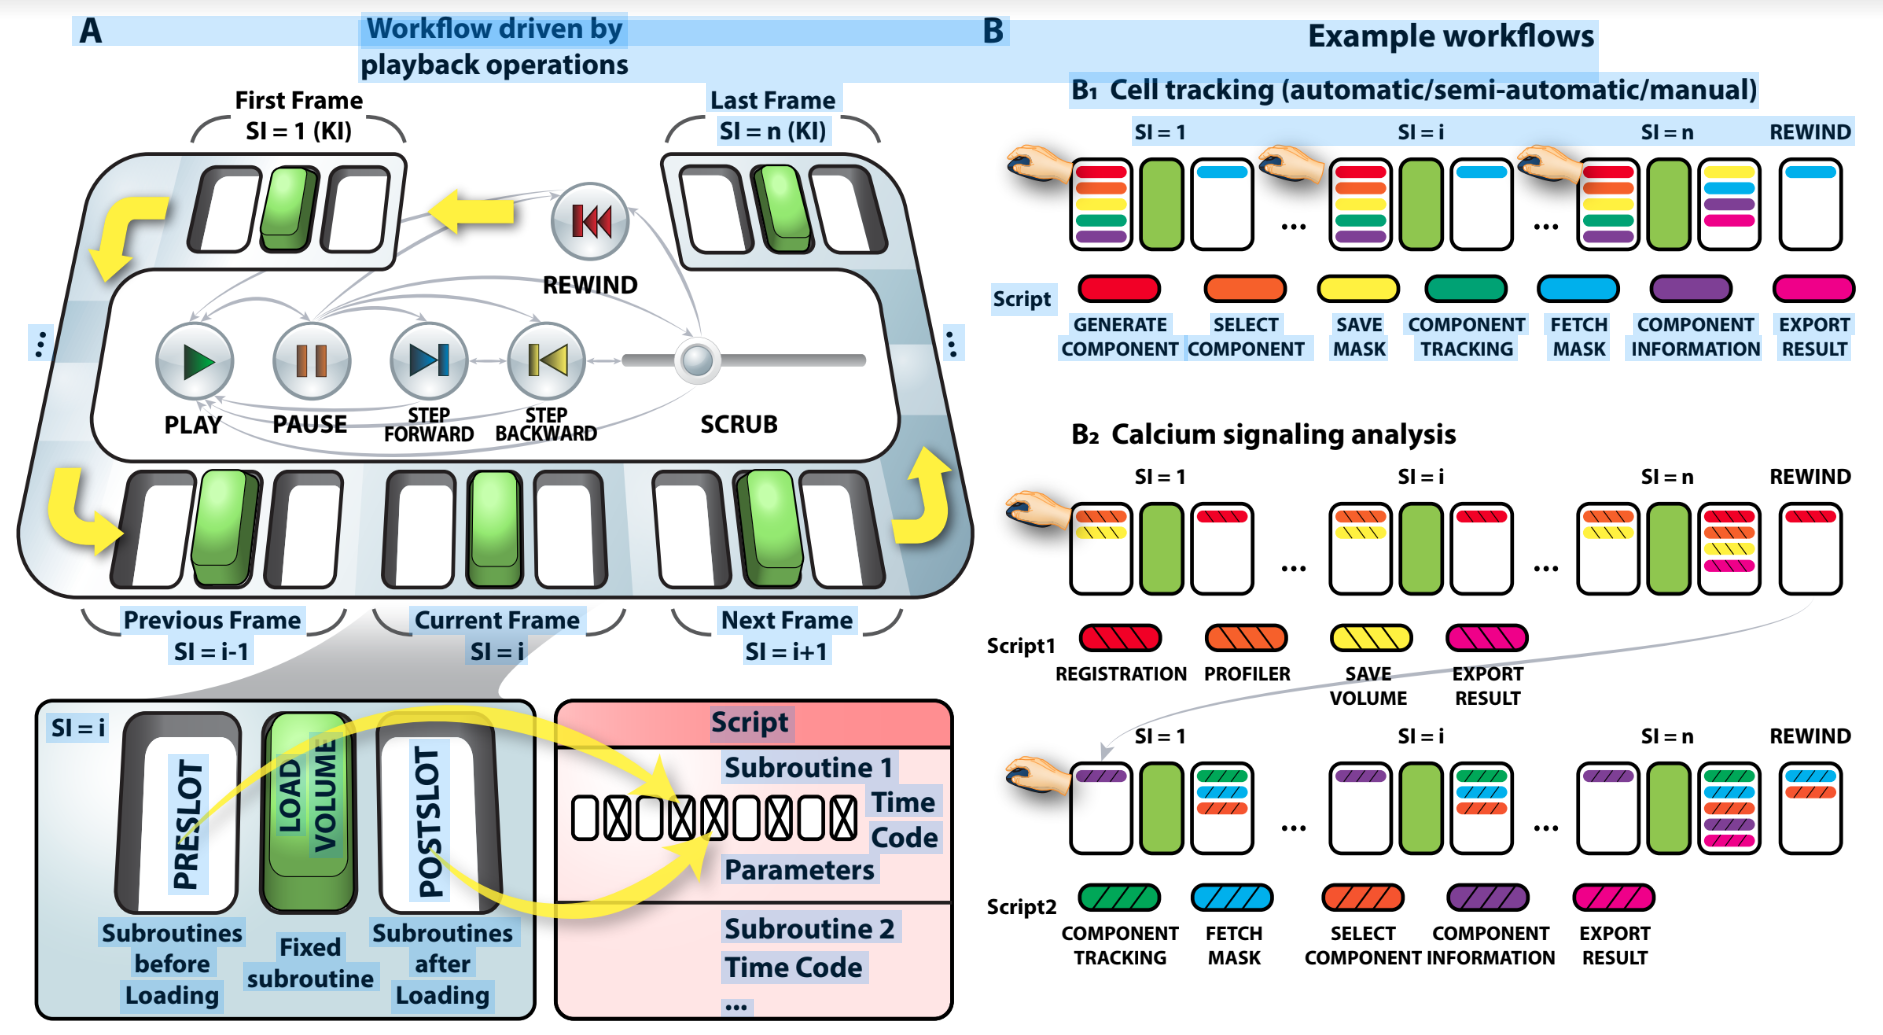
\includegraphics[width=26pc]{fig1.png}}
\caption{(A) The sequence index (SI) updates of a time-dependent sequence or an ensemble (size = n) are driven by the playback controls, which are extended to implement a general workflow. The operation orders of the playback controls, illustrated as the grey arrows, are well-understood by users. For each SI = i, LOAD VOLUME, shown as a green bar, is always executed. There are two slots, before and after this fixed subroutine, for workflow customization. All available subroutine slots are mapped into a time code as bits in a bit mask. Each subroutine in a script provides its time code for workflow assembly. (B) Two example workflows using this design for cell tracking and calcium signaling analysis. The hand icons indicate that semi-automatic and manual operations are intuitively supported when the playback is paused.\label{fig1}}\vspace*{-5pt}
\end{figure*}

\def\refname{REFERENCES}

\begin{thebibliography}{1}

\bibitem{one}
  C. Johnson, ``Translational computer science at the scientific computing and imaging institute,'' J. Comput. Sci., vol. 52, 2021.
\bibitem{two} J. C. Stockert and A. Blázquez-Castro, ``Fluorescence Microscopy in Life Science'', Sharjah: Bentham, 2017.
\bibitem{three} D. Abramson and M. Parashar, ``Translational research in computer science,'' Computer, vol. 52, no. 9, pp. 16-23, 2019.
\bibitem{four} R. P. Loui, ``In praise of scripting: real programming pragmatism,'' Computer, vol. 41, no. 7, pp. 22-26, 2008.
\bibitem{five} C. Brosch, ``On the conceptual history of the term lingua franca,'' J. Appl. Linguist. Stud., vol. 8, no. 1, pp. 71-85, 2015.
\bibitem{six} Y. Wan et al., ``FluoRender: joint free-hand segmentation and visualization for many-channel fluorescence data analysis,'' BMC Bioinform., vol. 18, p. 280, 2017.
\bibitem{seven} J. Wang and W. Tepfenhart, Formal Methods in Computer Science, Boca Raton: Chapman \% Hall, 2019.
\bibitem{eight} Y. Wan and C. Hansen, ``Independent and collaborative visualization tool development,'' IEEE Comput. Graph. Appl., vol. 39, no. 1, pp. 44-52, 2019.
\bibitem{nine} Y. Wan, H. Otsuna and C. Hansen, ``Synthetic brainbows,'' Comput. Graph. Forum, vol. 32, no. 3, pp. 471-480, 2013. 

\end{thebibliography}

\newpage

\begin{table}
\caption{Common subroutines in FluoRender script.\label{table1}}
\footnotesize
\centering
\begin{tabular*}{16.2cm}{|p{2cm}|p{2cm}|p{2cm}|p{2cm}|p{6cm}|}
\hline
SUBROUTINE & INPUT & OUTPUT & PARAMETERS & DESCRIPTION \\
\hline
Load Volume &
File on storage &
Volume &
Path to volume,\newline Channel index,\newline Time index &
Load one channel of volume at one time point from file. It is originally embedded within the playback of a volume sequence and not directly controlled by a script. \\ \hline

Fetch Mask & Volume &
Paint mask,\newline Component ID mask &
&
Fetch the paint mask or component ID mask for a volume from files on storage. The path to the file is deduced from the input volume. \\ \hline

Save Mask &
Volume,\newline Paint mask,\newline Component ID mask &
Mask files on storage &
&
Save masks associated with a volume as files on storage. A paint mask is usually generated from a user painting with a brush. A component ID mask can be automatically generated from image segmentation or manually specified by the user. \\ \hline

Render View Transformations &
Render view transformation &
Render view transformation   &
Render view UI &
An interactive subroutine, meaning its application is not controlled by the script and users can apply it at any time they see fit. \\ \hline

Paint Mask &
Volume,\newline Paint mask &
Paint mask &
Paint brush settings from UI &
An interactive subroutine. User paints with a brush tool and generates a volume mask, which is input to other subroutines. Masks constrain the computation on data only within the AOI defined by the mask. \\ \hline

Draw Rulers &
Volume &
Rulers &
Ruler settings from UI &
An interactive subroutine. Rulers are user-generated 3D vector graphics, usually for measuring distances. We also include landmark points as one type of ruler. Fluorescence intensity values can be sampled using rulers. \\ \hline

Generate Component &
Volume,\newline Paint mask &
Component ID mask &
Segmentation settings &
Segment a volume and assign each component from segmentation a unique ID. The IDs are stored in the component ID mask. The segmentation settings are directly retrieved from the UI, or from a macro recorded earlier, or from a database generated from machine learning. \\ \hline

Select Component &
Volume,Component ID mask &
Paint mask &
Selection mode,\newline Component size range &
Generate a paint mask from a component ID mask. Only segmented objects with component IDs are selected by the paint mask. A component size limiter is used to only select objects with specific sizes. \\ \hline

Profiler &
Volume,\newline Paint mask,
Rulers &
Intensity distribution of a volume on rulers &
Sample settings &
Sample fluorescence intensity values along rulers and generate a profile curve. \\ \hline

Component Information &
Volume,\newline Paint mask,\newline Component ID mask &
Intensity information on each component &
Component size range &
Compute information on each IDed component. The information includes those generated by the intensity distribution subroutine plus centroid coordinates, voxel count, physical volume, surface area, and major axis length from the principal component analysis. \\ \hline

Registration &
Source volume,\newline Target volume,\newline Paint mask &
Transformation information &
Initial search range,\newline Convergence criteria &
Transform the source volume to best match its fluorescence intensity to the target’s. \\ \hline

Component Tracking &
Volume,\newline Component ID mask &
Track graph &
Initial search range,\newline Convergence criteria &
Track individual components using the registration algorithm. The result is a graph that associates each pair of components from two time points. \\ \hline

Export Analysis Results &
Output from other subroutines &
Infographics &
Path to template,\newline Path to output file &
Compile and save analysis results in an HTML file, which is generated from a template with D3 support. The analysis results are usually directly presented to users with rich infographics at the end of executing a script. \\ \hline
\end{tabular*}
\end{table}

\end{document}

